\documentclass[conference]{IEEEtran}
\usepackage{amsmath}
\usepackage{graphicx}
\usepackage{booktabs}
\usepackage{url}
\newcommand{\SlowStdRatio}{237.4}
\newcommand{\FastStdRatio}{3.97}
\newcommand{\SlowPeakRatio}{612}
\newcommand{\FastPeakRatio}{3.54}
\newcommand{\StationaryZMean}{-1.0193}
\newcommand{\FastXMin}{-1.351}
\newcommand{\FastXMax}{1.268}

\newcommand{\ResultsRows}{%
Stationary & 0.000650 & 0.000636 & 0.000795 & 0.000354 & -- \\
Slow & 0.154299 & 0.030248 & 0.032058 & 0.216575 & 0.488 \\
Faster & 0.612748 & 0.138482 & 0.074244 & 0.767501 & 1.465 \\%
}

\begin{document}
\title{IMU Feature Extraction for Motion Analysis on Raspberry Pi Pico}
\author{\IEEEauthorblockN{Tanishq Vashishth}
\IEEEauthorblockA{UNI-ID: 266058IV\\IAS0360 -- Home Assignment 1\\Tallinn University of Technology}}
\maketitle

\begin{abstract}
This work implements statistical feature extraction and frequency analysis of acceleration on a Raspberry Pi Pico using an ICM-20948 sensor. Algorithms from the course laboratories were adapted to process real measurements in windows of 1024 samples at a target polling rate of 500 Hz. Three experiments compared a stationary board, slow repeated movement, and faster repeated movement. Eight complete windows were recorded per condition. The mean X-axis standard deviation increased from 0.000650 g at rest to 0.154299 g during slow movement and 0.612748 g during faster movement. The dominant X-axis frequency bin changed from 0.488 Hz to 1.465 Hz between the movement conditions. These observations demonstrate useful motion features, although they do not establish classification accuracy or a calibrated measurement of movement speed.
\end{abstract}
\begin{IEEEkeywords}
IMU, embedded signal processing, feature extraction, FFT, Raspberry Pi Pico
\end{IEEEkeywords}

\section{Introduction}
The objective was to implement laboratory signal-processing algorithms suitable for describing motion. Acceleration provides both information about the board's orientation relative to gravity and variation caused by movement. Statistical features summarize the amount of variation, while spectral features describe periodic components. All feature calculations run on the Pico; the computer records the output and prepares the comparison figures. A trained recognition model is outside the scope of this implementation.

\begin{table*}[t]
\caption{Comparison of all eight windows per condition. Values are arithmetic means of per-window features; frequency gives the observed range of X-axis peak bins across eight movement windows.}
\label{tab:results}
\centering
\begin{tabular}{lrrrrr}
\toprule
Condition & Mean $s_x$ ($g$) & Mean $s_y$ ($g$) & Mean $s_z$ ($g$) & Mean X peak amplitude ($g$) & X peak (Hz)\\
\midrule
\ResultsRows
\bottomrule
\end{tabular}
\end{table*}

\begin{figure*}[t]
\centering
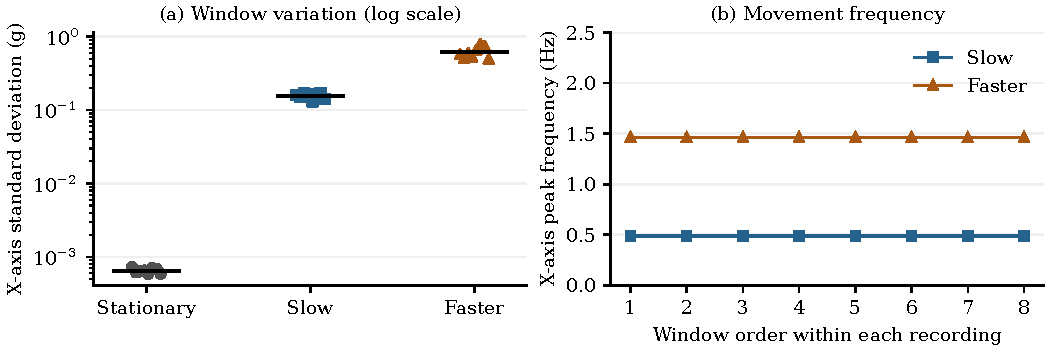
\includegraphics[width=\textwidth]{results_comparison.pdf}
\caption{Measured X-axis features. (a) Each dot represents one window; horizontal black marks indicate condition means. The vertical axis is logarithmic. (b) Peak frequency for slow and faster movement; window order is local to each recording, not shared time. Stationary peak frequencies are omitted because their very small amplitudes do not establish periodic motion.}
\label{fig:results}
\end{figure*}

\section{Hardware and Implementation}
The hardware is a Raspberry Pi Pico attached to the Waveshare Pico-Eval-Board, SKU 20159. This board contains an ICM-20948 motion sensor and an LCD~\cite{waveshare}. Only the accelerometer is used. The lab driver communicates through I2C1 on GP6 (SDA) and GP7 (SCL), at address 0x68. After lab initialization, checked register writes and readback set the accelerometer divider to zero, giving an internal output rate of 1125 Hz. The Pico polls at 500 Hz. The sensor retains the $\pm2g$ range and lab DLPF6 filter (about 5.7 Hz bandwidth); therefore, 500 Hz polling does not imply a 250 Hz signal bandwidth~\cite{tdk}. Signed readings are divided by 16384 to express acceleration in units of gravitational acceleration, $g$.

The implementation reuses the ICM-20948 initialization from Lab 1.1, statistical calculations from \texttt{statistic.c}, and the radix-2 FFT and Hamming window from \texttt{fft.c} in Lab 1.2~\cite{labs}. A checked six-byte read replaces the lab fast-read wrapper, avoiding its additional moving average. Static FFT scratch buffers keep the larger window off the Pico stack; processing runs on one core. The program collects three axes, computes their features separately, and prints one CSV row per axis through the Pico's USB connection. The LCD is not used in this experiment.

\subsection{Statistical Features}
For a window of $N=1024$ acceleration samples $a_n$, the mean, sample variance and standard deviation are
\begin{equation}
\mu=\frac{1}{N}\sum_{n=0}^{N-1}a_n,\quad
s^2=\frac{\sum_{n=0}^{N-1}(a_n-\mu)^2}{N-1},\quad s=\sqrt{s^2}.
\end{equation}
Minimum and maximum acceleration are also retained. These features are computed before windowing; consequently, the mean includes the contribution of gravity and sensor offset. Variance has units of $g^2$, whereas the other statistical features have units of $g$.

\subsection{Frequency Features}
The mean is removed before applying a Hamming window:
\begin{equation}
x_n=(a_n-\mu)\left[0.54-0.46\cos\left(\frac{2\pi n}{N-1}\right)\right].
\end{equation}
The FFT produces complex coefficients $X_k$. For positive-frequency bins below Nyquist, the amplitude is $A_k=2|X_k|/\sum_n w_n$, where $w_n$ is the Hamming window. The Nyquist bin uses a factor of one instead of two. The maximum-amplitude bin is selected from $k=1,\ldots,N/2$, excluding DC, and its frequency is $f_k=kf_s/N$.

The polling interval is 2 ms. A window represents approximately 2.048 s, with frequency-bin spacing $500/1024=0.48828125$ Hz. The effective polling rate is calculated from the first and last acquisition timestamps. Windows are rejected if a read fails or a scheduled acquisition is more than 200 microseconds late. Processing and printing occur between windows, so acquisition is not gap-free.

\section{Experiments and Verification}
The program was compiled in the course Docker environment, flashed onto the Pico, and exercised on the physical board. Host tests separately checked a constant signal, a sinusoid with a DC offset, sample variance, minimum and maximum, the expected FFT peak, and Nyquist amplitude scaling. The firmware build and these tests passed.

Three recordings were collected on September 26, 2026: the board resting on a surface, gentle repeated back-and-forth movement, and faster repeated movement. The varied experimental parameter was the manually applied movement rate. Polling rate, window length, sensor range and processing algorithms were held fixed. Motion distance and orientation were kept approximately similar by instruction but were not mechanically controlled or independently measured.

Each recording contains eight consecutive accepted windows: 34--41 for stationary, 72--79 for slow, and 98--105 for faster movement. The capture script discards its first encountered window to reduce transition contamination. Each condition provides 8192 sampled acceleration vectors and 24 feature rows, corresponding to 16.384 s of nominal sampled duration, excluding gaps. Across all conditions, 72 feature rows were validated for complete XYZ groups, finite values and consistent timing. Every retained row reports 500.000 Hz and minimum/maximum polling intervals of 2000 microseconds. These describe software polling, not independent sensor-clock accuracy.

\section{Results and Analysis}
Table~\ref{tab:results} summarizes every retained window rather than selecting individual examples. Figure~\ref{fig:results} shows the spread of X-axis variation and the stability of its selected frequency bin. X is emphasized because it has the largest standard deviation in both movement recordings; this is a descriptive choice, not a prevalidated classification rule.

At rest, the mean Z acceleration across windows was approximately $\StationaryZMean\,g$, consistent with gravity acting mainly along that axis together with alignment and sensor offset. The mean X standard deviation was only 0.000650 $g$. The small nonzero variation and spectral amplitudes are consistent with sensor noise and residual vibration; a peak frequency alone is insufficient evidence of periodic motion.

Slow movement increased the mean X standard deviation by approximately \SlowStdRatio{} times relative to rest, and its mean spectral peak amplitude by approximately \SlowPeakRatio{} times. The selected X frequency was 0.488 Hz in all eight windows. The statistical and frequency features therefore provide complementary evidence of repeated movement in this recording.

Faster movement increased the mean X standard deviation to 0.612748 $g$, approximately \FastStdRatio{} times the slow value. Mean peak amplitude increased by \FastPeakRatio{} times. Its frequency bin was consistently 1.465 Hz, corresponding to bin 3 rather than bin 1 in slow movement. This supports a higher repetition rate, but the precise physical rate was not independently measured. Acceleration amplitude also depends on movement distance and trajectory, so its increase cannot be attributed solely to repetition rate. The faster X readings ranged from $\FastXMin\,g$ to $\FastXMax\,g$, within the configured sensor range.

\section{Issues and Discussion}
The 0.488 Hz bin spacing limits frequency precision, and the Hamming window broadens spectral peaks while reducing leakage. The slow-motion peak is the first non-DC bin, corresponding to only about one cycle per window. It can be influenced by drift and gives a coarse repetition-rate estimate. Increasing $N$ to 2048 at 500 Hz would yield a calculated bin spacing of 0.244 Hz but require about 4.096 s of samples and additional memory. This is a design trade-off, not an additional measured experiment; no window-size or filter-parameter sweep was performed.

Manual movement introduces changes in displacement, orientation and force. Mean removal suppresses constant gravity/offset but does not compensate gravity when the board rotates. One session and eight windows per condition cannot establish general performance across users or activities. Independent repeated trials, a reference motion rate, and an amplitude threshold before reporting frequency would strengthen validation.

The retained data contain extracted features, not raw acceleration waveforms. Thus a new FFT configuration cannot be evaluated retrospectively from these files. Future firmware could log raw samples, use sensor data-ready interrupts or a FIFO, and buffer sampling while processing. The current polling and between-window pauses should be considered before use in continuous monitoring. Six-decimal CSV formatting also rounds some small stationary variances to zero; the nonzero standard deviations show that these are not exactly constant signals.

\section{Conclusion}
Lab-derived statistics, mean removal, Hamming windowing and FFT analysis were implemented and tested on the Pico with real IMU input. The recorded features distinguish the three tested motion conditions descriptively: acceleration variation increases with movement, and the faster recording has a higher dominant frequency bin. The source, complete recordings and reproducible analysis accompany this report.

\begin{thebibliography}{00}
\bibitem{waveshare} Waveshare, ``Pico-Eval-Board,'' product specifications, SKU 20159. [Online]. Available: \url{https://www.waveshare.com/pico-eval-board.htm}. Accessed: Sep. 26, 2026.
\bibitem{tdk} TDK InvenSense, ``ICM-20948 Datasheet,'' DS-000189, rev. 1.5, Table 18 and accelerometer sample-rate registers, 2021.
\bibitem{labs} Tallinn University of Technology, ``IAS0360 Lab Exercises 2026,'' Lab 1.1 IMU driver and Lab 1.2 statistics and FFT source files, course repository, 2026.
\end{thebibliography}
\end{document}
